\documentclass{cs0500}
\usepackage{xcolor}


\hwk{8}{Graph Algorithms - Part 1}{April 8, 2026 at 11:59 pm}

\usepackage{tikz}
\usepackage{graphicx}
\usepackage{pgfplots}
\tikzstyle{vertex}=[auto=left,circle,draw,minimum size=20pt,inner sep=0pt]

\begin{document}
\maketitle

    \begin{problem}
  In this question, we study single-source shortest paths with arbitrary edge weights. Consider the following directed graph H. The edge weights are labeled next to each edge. The source node is s = 0.

\begin{center}
    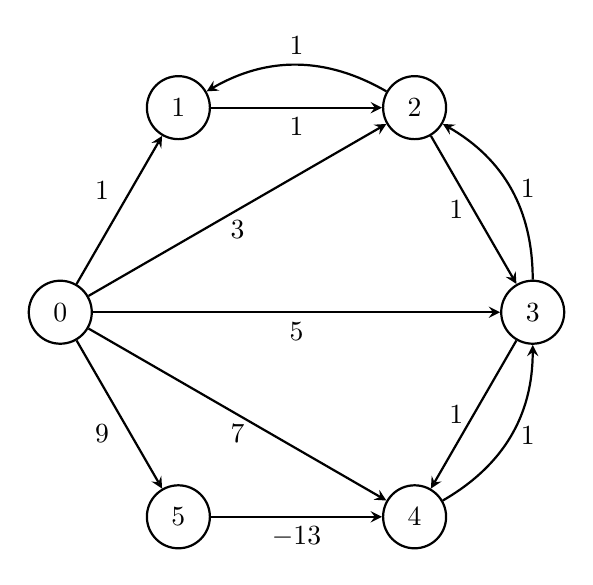
\begin{tikzpicture}[
    mynode/.style={draw, circle, thick, minimum size=0.8cm, inner sep=0pt},
    >={stealth},
    thick
    ]

    \node[mynode] (0) at (180:3) {0};
    \node[mynode] (1) at (120:3) {1};
    \node[mynode] (2) at (60:3) {2};
    \node[mynode] (3) at (0:3) {3};
    \node[mynode] (4) at (300:3) {4};
    \node[mynode] (5) at (240:3) {5};


    \draw[->] (0) -- node[above left] {1} (1);
    \draw[->] (0) -- node[below] {3} (2);
    \draw[->] (0) -- node[below] {5} (3);
    \draw[->] (0) -- node[below] {7} (4);
    \draw[->] (0) -- node[below left] {9} (5);    
    \draw[->] (1) -- node[below] {1} (2);
    \draw[->] (2) to[bend right=30] node[above] {1} (1);
    \draw[->] (2) -- node[left] {1} (3);
    \draw[->] (3) to[bend right=30] node[right] {1} (2);    
    \draw[->] (3) -- node[left] {1} (4);
    \draw[->] (4) to[bend right=30] node[right] {1} (3);
    \draw[->] (5) -- node[below] {$-13$} (4);

\end{tikzpicture}
\end{center}

\begin{enumerate}[(a)]
    \item \textbf{Dijkstra's Algorithm:} Run Dijkstra's algorithm on $H$. Write down the order in which nodes are finalized and the distances $d(v)$ returned. What do you observe?
    \item \textbf{Bellman-Ford Algorithm:} Let $OPT(i, v)$ be the length of the shortest path from $s$ to $v$ using at most $i$ edges. Complete the table below.

    \begin{center}
    \begin{tabular}{@{}ccccccc@{}}
    \toprule
    $i \setminus v$ & 0 & 1 & 2 & 3 & 4 & 5 \\ \midrule
    0 & 0 & $\infty$ & $\infty$ & $\infty$ & $\infty$ & $\infty$ \\
    1 &   &   &   &   &   &   \\
    2 &   &   &   &   &   &   \\
    3 &   &   &   &   &   &   \\
    4 &   &   &   &   &   &   \\
    5 &   &   &   &   &   &   \\ \bottomrule
    \end{tabular}
    \end{center}
\end{enumerate}
 
\end{problem}
\begin{solution}
\end{solution}
\pagebreak
\begin{problem}[Maximum Bottleneck Path]
You are given a graph $G = (V, E)$ with $n$ vertices and $m$ edges, represented as an adjacency list.
Each edge $e = (u,v) \in E$ has a nonnegative capacity $c(e)$.
Given two vertices $s, t \in V$, a path $P$ from $s$ to $t$ has
\emph{bottleneck capacity}
\[
\text{bottleneck}(P) = \min_{e \in P} c(e).
\]
\begin{enumerate}[(a)]
    \item  Describe an algorithm that, given as input $G=(V,E)$ and a starting vertex $s$, finds for all vertices $v\in V$ a path from $s$ to $v$ whose bottleneck capacity is as large as possible. If for a vertex $v$ no such path exists from $s$ to $v$, the algorithm should return $d[v]=0$. Your algorithm should run in $\mathcal{O}((|V|+|E|)\log |V|)$ time.
\item Provide a proof of correctness of your algorithm.
    \item Provide a proof of the running time of your algorithm.
    \item Analyze how much memory space your algorithm is using in excess of the memory space used to represent the input. 
\end{enumerate}
\medskip
\noindent \textbf{Hint.}
Consider modifying Dijkstra's algorithm.

\end{problem}
\begin{solution}  
\end{solution}
\pagebreak
\begin{problem}[Shortest Paths with Alternating Colors]
You are given a directed graph $G$ on nodes $0,1,\dots,n-1$, represented as an adjacency list. Each edge is assigned a weight $w(u,v)$ and a color attribute from the set $\{{\color{red} red}, {\color{blue} blue}\}$. 
Edges with the {\color{red} red} attribute are called {\color{red} red edges} and edges with the {\color{blue} blue} attribute are called {\color{blue} blue edges}.
Note that there may be both a {\color{red} red edge} and a {\color{blue} blue edge} connecting the same pair of edges, even in the same direction. These edges may have different weights.

A directed path is said to be \emph{alternating colors} if consecutive edges in it are of different colors. The weight of one such alternating color path is the sum of the weights of its edges.

An \emph{alternating color directed cycle} is an alternating color from a vertex to itself. In $G$, there are no alternating color directed cycles whose weight is negative.
\begin{enumerate}[(a)]
    \item Describe an algorithm that, given as input $G=(V,E)$ and a starting vertex $s$, computes for all vertices $v$ the minimum cost of an alternating color path from $s$ to $v$. If for a vertex $v$ no such path exists, the algorithm should return $d[v]=\infty$. Your algorithm should run in $\mathcal{O}(|V||E|)$ time.
    \item Provide a proof of correctness of your algorithm.
    \item Provide a proof of the running time of your algorithm.
    \item Analyze how much memory space your algorithm is using in excess of the memory space used to represent the input. 
\end{enumerate}

\end{problem}

\begin{solution}
\end{solution}

\end{document}
